\documentclass{aa} 

\usepackage{natbib}
\usepackage{graphicx}
\usepackage{color}
\usepackage{txfonts}
% If it won't compile, set or remove draft mode
%\usepackage{hyperref}       
\usepackage[draft]{hyperref} 
\usepackage[T1]{fontenc}
\usepackage{verbatim}
\usepackage{upgreek}
\usepackage{float}


%________________________________________________________________

\newcommand{\brgamma}{\ion{Br}{$\gamma$}~}
\newcommand{\sig}{$\sigma$~}
\newcommand{\m}{$^\mathrm{m}$~}
\newcommand{\micron}{\upmu\mathrm{m}}

%________________________________________________________________

\newcommand{\occomment}[1]{\textbf{\textcolor{red}{(OC: #1)}}}
\newcommand{\klcomment}[1]{\textbf{\textcolor{green}{(KL: #1)}}}

\begin{document} 

  \title{SimCADO I: Introducing the instrument data simulation suite for MICADO at the ELT}
  %\subtitle{}
  \author{K. Leschinski\inst{1}
     \and
          O. Czoske\inst{1}
     \and
          G. Verdoes Kleijn\inst{2}
     \and     
          R. Davies\inst{3}
     \and
          W. Zeilinger\inst{1}
     \and
          J. Alves\inst{1}
      }
     

  \institute{Department of Astrophysics, University of Vienna,
          Türkenschanzstr.~17, A-1180 Vienna, Austria\\
          \email{kieran.leschinski@univie.ac.at}
%     \and
%         Institut für Astro- und Teilchenphysik, Universität Innsbruck, Technikerstr.~25/8, A-6020 Innsbruck, Austria
     \and
         Kapteyn Astronomical Institute, University of Groningen, PO Box 800, 9700 AV Groningen, The Netherlands
     \and
         Max Planck Institute for Extraterrestrial Physics, PO Box 1312, D-85741 Garching, Germany
      }

  \date{Received 01.03.2018; accepted TBD}

  \abstract
% context heading (optional)
% {} leave it empty if necessary
% {When the Extremely Large Telescope comes online at the end of 2025, MICADO will be the near infrared imaging camera available at first light. As part of the design activities for MICADO we have developed SimCADO: an instrument data simulator in the form of a Python package. SimCADO produces simulated data frames for MICADO's nine detector chips by applying the effects of each element along the optical train to a three dimensional ($x$, $y$, $\lambda$) description of the flux arriving from an astronomical object. Simulated images can be written to disk as FITS files and can be analysed by the standard suite of astronomical software.}
% aims heading (mandatory)
% {The main aims of this paper are two fold: to introduce the SimCADO software, and to provide preliminary detection limits for MICADO based on SimCADO simulations. By presenting these limits we also aim to raise awareness in the community of the future capabilities of MICADO and the current capabilities of SimCADO.}
% methods heading (mandatory)
% {To verify the accuracy of SimCADO we compared the characteristics of simulated images of globular clusters with images of the same clusters from the ESO archive. We then used a model of the current optical train design for MICADO to determine the sensitivity limits for MICADO at the ELT.}
% results heading (mandatory)
% {SimCADO is able to accurately reproduce the image characteristics of raw archival HAWK-I data to within the limits of the model of the UT4/HAWK-I optical train. Using the current design of MICADO, SimCADO finds detection limits in the J, H and Ks filters to be 28.7\m, 27.9\m and 27.3\m (Vega) respectively for a $5\sigma$  detection in a 5 hour observation. This leads to the ability to observe for the first time with a ground based observatory individual A0\,V stars at a distance of 4\,Mpc (i.e. in \object{Centaurus A}), and M9\,V stars in the \object{Large Magellanic Cloud}.}
% conclusions heading (optional), leave it empty if necessary 
% {}
{}
{MICADO will be the first-light near-infrared imaging camera at ESO's extremely large telescope. As part of the design activities for MICADO we have developed SimCADO: an instrument data simulator in the form of a Python package (\url{https://simcado.readthedocs.io/}.}
{To verify that the images produced by SimCADO are realistic in terms of both flux levels and spatially dependent optical artifacts we configured the software to mimic the HAWK-I/VLT-UT4 optical system. The characteristics of simulated HAWK-I images of two globular clusters compared very favourably with actual observations taken from the ESO archive. This confirmation of the software's accuracy allowed us to confidently make predictions about the point source sensitivity of MICADO at the ELT.}
{We find that the $5\sigma$ limits for a 5 hour SCAO observation in the J, H, and Ks filters are around 29.6$^m$, 29.3$^m$ 29.1$^m$ in the AB magnitude system. Furthermore we provide simple observation horizons for a series of stellar spectral types for a range of total exposure time and in the J and Ks filters.}
{}


  \keywords{}

\maketitle

%________________________________________________________________

\section{Introduction}
\label{sec:Introduction}

Over the next decade the era of the extremely large telescopes will be begin.
The European Extremely Large Telescope \citep[ELT, ][]{eelt} will provide astronomers with the increase in resolution and sensitivity needed to solve many of the outstanding questions of modern day astronomy. 

With a 39\,m primary mirror consisting of 798 individually steerable 1.45\,m hexagonal mirror segments and a fully deformable quaternary mirror, the ELT will be capable of providing diffraction-limited imaging with the help of the adaptive optics (AO) modules.
This corresponds to a core full-width half maximum (FWHM) for the point spread function (PSF) in the J-band ($1.2\,\micron$) of $8\,\mathrm{mas}$ and $14\,\mathrm{mas}$ in the Ks-band ($2.16\,\micron$).
Both single- and multi-conjugate modes for the adaptive optics will be possible.
Laser guide stars (LGS) will be available to ensure that the ELT will always be able to provide AO-assisted observations. 

As the first-light wide-field imaging camera for the ELT, MICADO -- the \textbf{M}ulti-AO \textbf{I}maging \textbf{CA}mera for \textbf{D}eep \textbf{O}bservations \citep{micado} -- will take advantage of the ELT's near-infrared optimised design to provide images at the diffraction limit.
MICADO will provide a wide-field imaging mode and a zoom (narrow-field) mode with 4\,mas/pixel and 1.5\,mas/pixel plate-scales respectively.
The detector plane will consist of nine $4096\times 4096$ detector chips, allowing MICADO to cover a Field of View (FOV) of $\sim55\arcsec$ by $50\arcsec$ in the wide-field mode and $21\arcsec$ by $19\arcsec$ in the high resolution mode.

MICADO will also contain a series of additional modes, including: a long-slit spectrographic mode with a spectral resolution of up to $R\sim20\,000$ for point sources and $R\sim8000$ for extended sources, and a high-contrast imaging mode.

As the scale and complexity of telescopes and instruments increases, so too does the importance of accurately being able to predict the performance of these systems.
More and more emphasis is being placed on developing simulation software to model new instruments before they enter the construction phase.
As part of the development of the MICADO instrument, the MICADO Data Flow System (DFS) team has been tasked with creating a tool to simulate raw detector read-out images based on the current designs of the ELT and MICADO.
Here we present SimCADO, the instrument data simulator for MICADO. 

SimCADO combines the most recent data from the other work packages in the consortium to allow the user to simulate the above mentioned raw data frames as will be produced by the ELT/MICADO optical system.
Originally conceived as a tool to aid the development of the data reduction pipeline, SimCADO has also found use among the science team as a way of conducting feasibility studies for various future observations.

Section \ref{sec:simcado} breifly describes where SimCADO can be found.
In section \ref{sec:hawki} we present the validation tests for the software using a model of HAWK-I at the VLT.
The current best estimates for the sensitivity limits of MICADO are presented in Section \ref{sec:predictions}, followed by estimates of the observational horizons for main sequence stars.
In Section \ref{sec:future} we outline the functionality to be included in future versions of the software.

% In this paper we briefly introduce the SimCADO package and show that it is a useful tool for producing not only accurate simulated images for the MICADO/ELT optical system, but also for any other optical train, such as for HAWK-I on UT4 at the VLT. It should be noted that the design of SimCADO is described in detailed in \citet{leschinski2016}. Aspects which have been updated in the mean time are detailed in this paper. For all other design aspects the reader should still consult \citet{leschinski2016}. This paper is organised in the following way: Sect.~\ref{sec:scope} delves briefly into the motivation behind creating SimCADO as well as giving an overview of the scope of the project. The physical effects that SimCADO models are described in Sect.~\ref{sec:simcado}. A description of how we validated SimCADO by comparing simulated VLT/HAWK-I read-out frames to real images from the ESO archive can be found in Sect.~\ref{sec:hawki} and predictions for the sensitivity of the ELT/MICADO system are presented in Sect.~\ref{sec:predictions}. A discussion of the results, assumptions and issues with the simulated images is presented in Sect.~\ref{sec:discussion}.

\section{SimCADO -- the Python package for simulating MICADO observations}
\label{sec:scope}


\subsection{Code availability}


The astronomy community appears to be very much in line with the general trend in the scientific community towards using the Python language for scientific computing purposes. As such the SimCADO package has been made for the Python ecosystem. Documentation for using SimCADO can be found on Read the Docs (\url{https://simcado.readthedocs.io}). The package is available via the python package index (PyPI) and can be installed using the standard command:\\

\verb+pip install simcado+\\

The code is open source and publicly available for cloning at the author's GitHub repository: \url{https://github.com/astronomyk/SimCADO}. 

SimCADO is capable of simulating the readout images from the 9 HAWAII-4RG detectors in the MICADO focal plane and simulates the effect of various optical and mechanical elements, e.g: the field varying nature of the point spread function (PSF), atmospheric dispersion and spectral characteristics, residual field rotation from the derotator, transmission losses and thermal emission from all optical surfaces, the effects of non-common path aberrations on the system transmission, correlated and uncorrelated detector noise, detector linearity and saturation effects, photon shot noise, etc. For a full list of effects in the package, the reader is directed to see the online documentation, or to refer to \citet{leschinski2016} for more details. The online documentation also provides several tutorials and worked examples to help the user get started with the package.

While originally conceived as a way to mimic the telescope data environment for the purposes of developing the data reduction pipeline, SimCADO has also been adopted by the MICADO science team as a tool for conducting scientific and observational feasibility studies. The results of some of these feasibility studies will be presented in future papers. The remainder of this paper is dedicated to showing how we validated the accuracy of SimCADO simulations against raw HAWK-I/VLT images, and what that means for the predicted sensitivity of MICADO/ELT.



\section{Validating SimCADO by modelling the VLT/HAWK-I optical system}
\label{sec:hawki}

Aside from testing during the coding phase, we tested the accuracy of SimCADO by comparing simulated raw detector readout images to raw observations from HAWK-I on UT4 at the VLT. HAWK-I, the High Acuity Wide-field K-band Imager \citep{hawki}, is a present-day analogue to MICADO's imaging modes and thus a good test-bed for these comparisons. In order to create a version of SimCADO that simulates raw observations for the VLT/HAWK-I optical train, we created a simulation configuration file that reflects the UT4/HAWK-I optical train from the publicly available instrument data on the ESO website\footnote{\url{http://www.eso.org/sci/facilities/paranal/instruments/HAWK-I.html}} and from HAWK-I calibration data from the ESO archive. The verification process included two tests on the simulated output data. The first tested whether the HAWK-I version of SimCADO could reproduce the sensitivity limits of the VLT/HAWK-I system as given in \citet{hawki}. The second involved simulating images of two globular clusters and comparing them against the real images from the ESO archive. The raw images used for the comparison were several J and Ks images of the globular clusters M\,4 and NGC\,4147, downloaded from the ESO archive.

\subsection{Modelling HAWK-I with SimCADO}

To create a model of the HAWK-I optical train, SimCADO required the following data:
\begin{itemize}
    \item an estimate of the Point Spread Function (PSF) for the whole VLT/HAWK-I system,
    \item transmission/reflectivity curves for each of the surfaces along the optical path, 
    \item details of the HAWAII-2RG detector characteristics
\end{itemize}

Additionally, a description of the globular clusters to be observed was needed. Creating the descriptions of the on-sky sources is described in more detail in Sect.~\ref{subsec:HAWKI_comparison}.

\paragraph{The point spread function (PSF):}
The seeing-limited nature of the UT4/HAWK-I optical train greatly simplified simulations. The combined system PSF can be described by a diffraction limited Moffat profile for the round monolithic mirrors of the UT4 telescope \citep{vlt_mirror} combined with a Gaussian profile for the atmospheric contribution. We used the POPPY package \citep{poppy} to generate a diffraction limited PSF for an 8.2\,m circular aperture with a 1.1\,m secondary obscuration and four support beams with a width of 0.1\,m. We then convolved this diffraction-limited PSF with a $0.5\arcsec$ 2D Gaussian profile to mimic the seeing-limited nature of HAWK-I observations. This artificial PSF can be seen in the bright stars in the right image of Fig.~\ref{fig:img_comparison}.

\paragraph{Transmission curves for the optical train:}
The combined optical train of HAWK-I and the VLT's UT4 contains 7 aluminium-coated mirrors, an entrance window, a series of standard NIR filters and a detector plane with four~HAWAII-2RG detectors. The transmission, reflectivity and quantum efficiency curves for each of these elements were combined in SimCADO. The resulting transmission curve has an average transmission value of 0.52, which is very similar to the average value of 0.5 assumed by the online exposure time calculator provided by ESO.\footnote{\url{https://www.eso.org/observing/etc/bin/simu/HAWK-I}}

\paragraph{The detector array:}
Four HAWAII-2RG detectors \citep{hawaii2rg} make up the HAWK-I detector plane. The detector noise was generated internally by SimCADO using the NGHxRG package \citep{nghxrg}. The quantum efficiency curve was taken from \citet{finger2008}. The detector linearity curve was extracted from the Ks-band archive image \verb+HAWK-I.2015-06-10T05_12_28.683+. It was determined by fitting Gaussian profiles to the wings of a series of saturated stars in the raw observations and comparing the theoretical height of the best-fit Gaussian profile to the actual pixel values in saturated regions. The plate scale used by SimCADO was $0.106\arcsec$, as reported by \citet{hawki}.

%Instrumental distortion was neglected because its effect was minimal when determining the photometric accuracy of a simulated stellar field. 
The flat field effect of the whole system was neglected for these tests. The archive images were not flat field corrected, and no flat field was applied to the simulated images. This decision was made because the vast majority of the stars in the globular clusters were located in the central region of the image where the variable field illumination plays a negligible role with respect to the photometric accuracy.

%It should be noted that we are in the process of conducting a further study to quantify the extent to which different atmospheric conditions affect the accuracy of images generated with SimCADO. For this study we were granted 5~hours of technical time on HAWK-I and will report on the results in a future paper. 


\subsection{Test 1 - HAWK-I Sensitivity with SimCADO}

\begin{table}
    \centering
    \caption{Limiting Vega magnitudes calculated for HAWK-I from images generated by SimCADO, the ESO ETC and taken from \citet{hawki}. The SimCADO limiting magnitudes were calculated based on a $5\sigma$ detection in a grid of 100 stars with magnitudes spread linearly between 14\m and 27\m in the respective filters. The FWHM for the SimCADO PSF was chosen to match the ``Image Quality'' parameter given by the ETC. For a seeing value of $0.8\arcsec$ in V band and an airmass of 1.2, the resulting FWHM for J, H, and Ks (\brgamma) band respectively was $0.62\arcsec$, $0.58\arcsec$, $0.53\arcsec$.}
    \label{tab:HAWKI_lim_mags}
    \begin{tabular}{ l  r r r r }
    \hline\hline
    Filter & Exposure  & SimCADO          & ETC                &  KP+2008 \\
           &           & (Vega)           & (Vega)            & (Vega)  \\
    \hline
           & 1 hr           &  23.8\m          &  24.2\m            &  23.9\m          \\
    J      & 1 min          &  21.5\m          &  22.0\m            &                    \\
           & 2 sec          &  19.7\m          &  20.1\m            &                    \\
    \hline
           & 1 hr           &  22.7\m          &  23.3\m            &  22.5\m          \\
     H     & 1 min          &  20.5\m          &  21.0\m            &                    \\
           & 2 sec          &  18.8\m          &  19.2\m            &                    \\
    \hline
           & 1 hr           &  21.9\m          &  22.2\m            &  22.3\m          \\
    Ks     & 1 min          &  19.7\m          &  19.9\m            &                    \\
           & 2 sec          &  17.8\m          &  18.1\m            &                    \\
    \hline
   	       & 1 hr           &  21.6\m          &  20.9\m            &                    \\
\brgamma   & 1 min          &  19.5\m          &  18.7\m            &                    \\
           & 2 sec          &  17.5\m          &  16.8\m            &                    \\
    \hline
    \end{tabular}

\end{table}

As a first test we compared the limiting magnitudes of images generated with SimCADO to both the limiting magnitudes given by \citet{hawki}, and those given by the exposure time calculator (ETC) on the ESO website. For the SimCADO model of HAWK-I we determined the limiting magnitudes by simulating images of a grid of 100 stars with magnitudes ranging from 15\m to 27\m in each of the HAWK-I filters. The grid was ``observed'' for a series of exposure times ranging from 2\,seconds to 1~hour. As the positions of the stars were known, we used aperture photometry to calculate the signal to noise ratio (SNR) for each of the stars in each of the exposure and filters. The limiting magnitude for image was set by the star with a SNR closest to, but not lower than $5\sigma$. The results for various exposure times are shown in Table \ref{tab:HAWKI_lim_mags} and for the J-band in Fig. \ref{fig:HAWKI_rainbow_j}.

It can be seen from Table~\ref{tab:HAWKI_lim_mags} that the limiting magnitudes for SimCADO in the J and H filters are within 0.2\m of the values given by \citet{hawki}, although there is a $\sim$0.5\m discrepency between SimCADO and the ETC. In the Ks filter the discrepancy is only $\sim$0.3\m. The \brgamma filter shows the biggest deviation of $\sim$0.7\m. The observation parameters used in SimCADO were set to be identical to those described by \citet{hawki}, namely: seeing of $0.8\arcsec$ in V-band and an airmass of 1.2. Fig.~\ref{fig:HAWKI_rainbow_j} shows the evolution of several relevant detection limits (e.g.\ $5\sigma$ for photometry, $\sim 250\sigma$ for astrometry) for HAWK-I as determined by SimCADO.


\begin{figure}

    \centering
    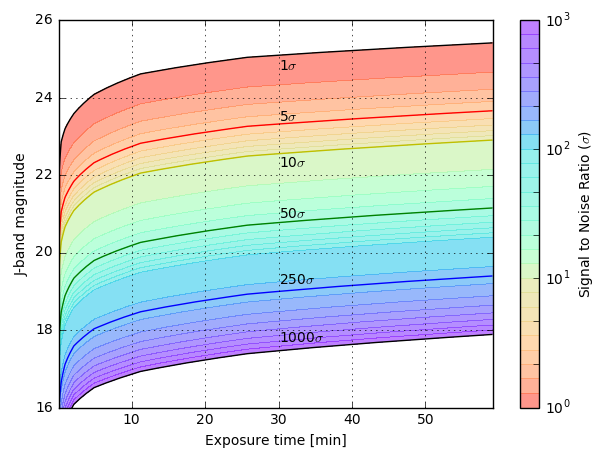
\includegraphics[width=0.48\textwidth]{images/HAWKI_SNR_Rainbow_J}
    
    \caption{Limiting Vega magnitudes as predicted by SimCADO for the UT4/HAWK-I optical system. A grid of hundred stars were observed for different durations between 1 and 60 minutes using SimCADO configured to model UT4/HAWK-I. The $5\sigma$ contour in this graph is $\sim 0.5$\m lower than the theoretical $5\sigma$ detection limits as returned by the ESO HAWK-I ETC. However the one hour $5\sigma$ Vega magnitude limit ($J=23.7$\m) is within 0.2\m  of the limit published by \citet{hawki}.}
    \label{fig:HAWKI_rainbow_j}

\end{figure}


\subsection{Test 2 - Comparison of SimCADO images with real observations}
\label{subsec:HAWKI_comparison}

\begin{table*}

    \centering
    \caption{The raw un-reduced HAWK-I data from the ESO archive used in this study. The three observations of M\,4 were used to test the photometric accuracy of SimCADO under the assumption that the background flux level remained similar. The observation of NGC\,4147 was used to test the background flux for different length exposures.}
    \label{tab:HAWKI_raw}
    \begin{tabular}{c c c c c c }
        \hline\hline
        ESO archive filename                        & Filter & Exposure [s] & V-band seeing [arcsec]    &  Airmass  & Object  \\
        \hline
        \verb+HAWK-I.2015-06-10T05_12_28.683.fits+   & Ks     &  10          &  0.9                      &  1.05     & M\,4    \\
        \verb+HAWK-I.2007-08-05T01_34_45.908.fits+   & Ks     &  10          &  NA                       &  1.05     & M\,4    \\
        \verb+HAWK-I.2007-08-05T23_14_33.748.fits+   & J      &  10          &  1.1                      &  1.02     & M\,4    \\
        \hline
        \verb+HAWK-I.2014-01-19T07_49_48.826.fits+   & J      &  2           &  0.74                     &  1.44     & NGC\,4147    \\
        \hline
    \end{tabular}
    
\end{table*}


To test how well SimCADO reproduces the spatial aspects of an observation, we downloaded four raw FITS files of the globular clusters M\,4 and NGC\,4147 from three different observing runs conducted between 2007 and 2015 from the ESO archive. Table~\ref{tab:HAWKI_raw} lists the main parameters of these observations. Globular clusters by virtue of their age contain very little gas or dust and hence essentially no star formation activity. This makes them easy objects to model for SimCADO. We chose this series of raw images to test the performance of SimCADO over multiple observing configurations. 

\begin{figure}

    \centering
    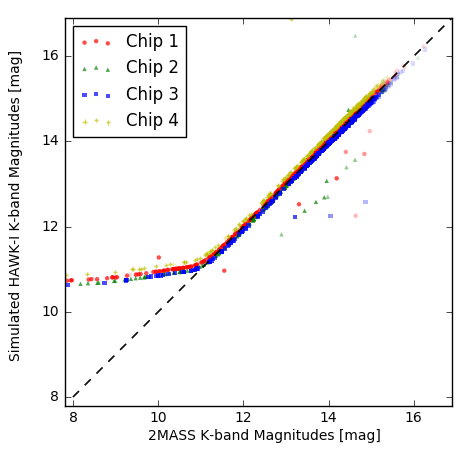
\includegraphics[width=0.45\textwidth]{images/2MASS_vs_HAWKado_inst_mags_single}
    
    \caption{Instrumental K-band magnitudes (Vega) from an observation of M\,4 simulated with SimCADO (SimCADO output) versus K-band magnitudes (Vega) from the 2MASS catalogue (SimCADO input). The one-to-one correlation was to be expected because the brightness levels of the stars in the simulated images were based on the 2MASS catalogue. The cloud of points below the line shows where two stars were close enough together that the pipeline chose the wrong star. It was set up to choose the brightest star within a $1\arcsec$ radius around each coordinate in the 2MASS catalogue. The deviation from the one-to-one line around $K_{s}=11$\m is due to SimCADO reproducing the saturation characteristics of the HAWK-I detector. The effect of the different gain values for the HAWK-I detectors is also visible as the slight offset between the different coloured dots. The instrumental zero-point used was 27.2\m.}
    \label{fig:2mass_hawkado_flux_comparison}

\end{figure}

\begin{figure*}

    \centering
    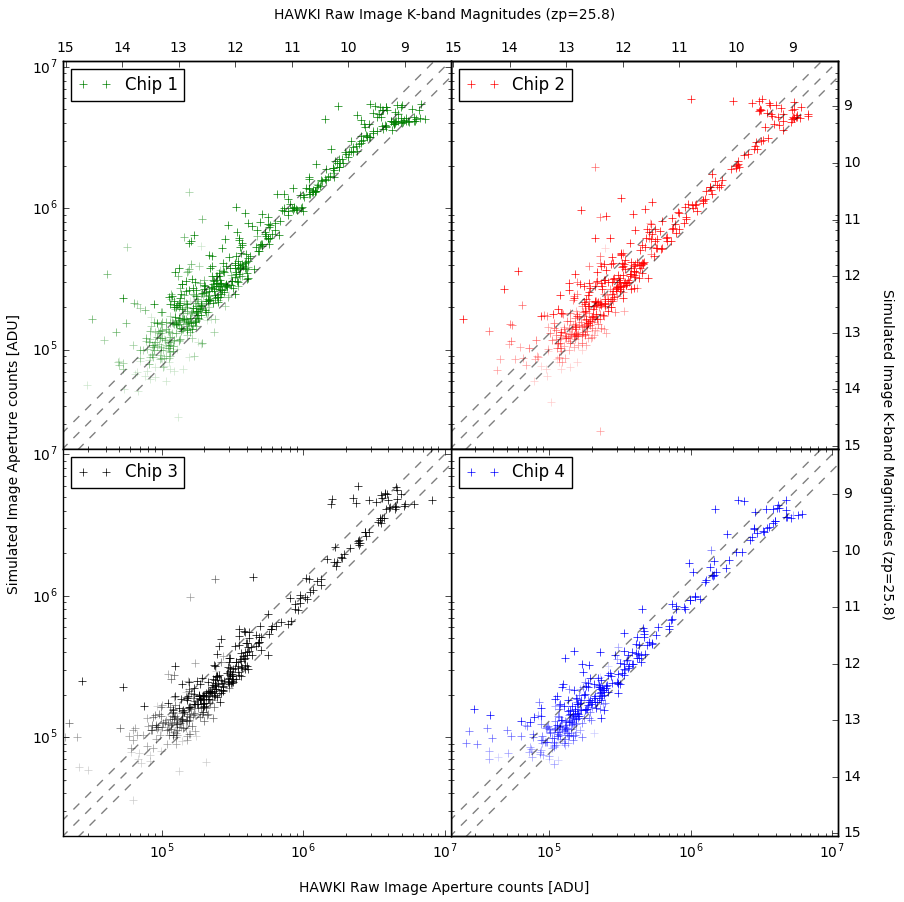
\includegraphics[width=\textwidth]{images/HAWKI_vs_HAWKado_couts_and_mags.png}
    
    \caption{Flux counts from aperture photometry of the stars in the simulated and real Ks-band images of M\,4. Each detector is plotted separately here as they cover different regions of M\,4 and have different gain factors. The strength of the symbols is determined by the photometric quality flag in the 2MASS catalogue. The dashed lines are the $\pm 0.3^\mathrm{m}$, or 30\,\% flux difference intervals. For detectors~1 and~2  more than 75\,\% of stars with A-grade 2MASS photometry fall within these bands. For detectors~3 and~4 this is $>85\,\%$. Approximately 55\,\% of the sources with C-grade or worse 2MASS photometry flags fell outside the $\pm 30\,\%$ bands. When investigating these sources we found a large fraction to be single entries in the 2MASS catalogue, were resolved into multiple stars in the HAWK-I images. Photon statistics only play a role for aperture fluxes on the order of $10^{4}$ counts.}
    \label{fig:HAWKI_hawkado_flux_comparison}
    
\end{figure*}

\begin{figure*}

    \centering
    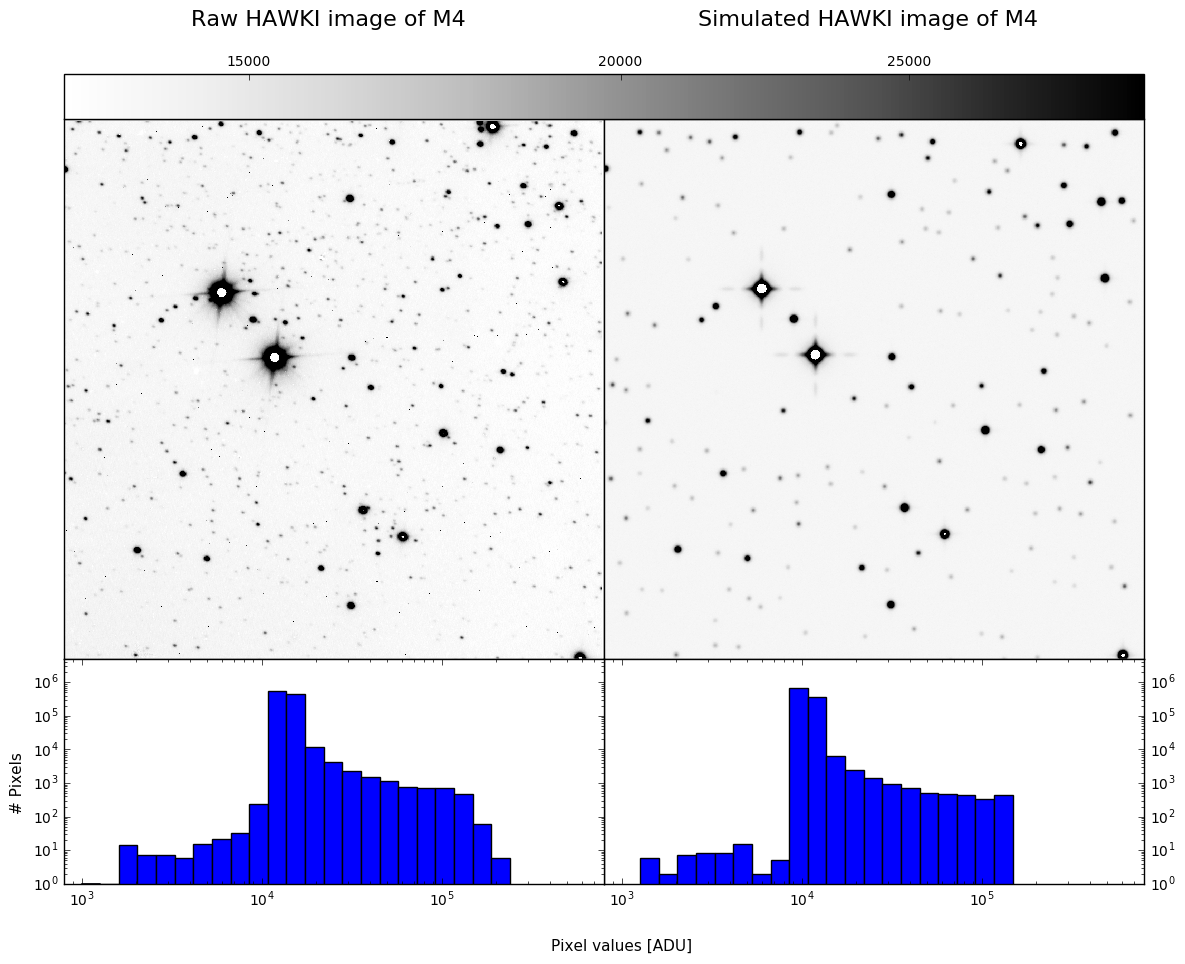
\includegraphics[width=\textwidth]{images/hawki_simcado_side_by_side}
    
    \caption{Top: A comparison of a raw HAWK-I image (left) with a simulated image (right) from SimCADO for the same field near M\,4. The 2MASS point source catalogue was used to populate the simulated images. As such no sources fainter than the 2MASS detection limit were included. Features created by the optical train (e.g.~diffraction spikes) and by the detector (e.g.~saturation) can be seen in both the real and simulated images. The apparent size of the PSF for the brightest stars in the simulated images is smaller than in the real images because SimCADO does not currently model leakage from saturated pixels into neighbouring pixels. Bottom: The distribution of pixel counts for the real (left) and simulated (right) images is given here to illustrate that SimCADO is capable of recreating observations with no ``real world'' input. The discrepancy in the shape of the histogram for pixel counts less that 10\,000 is due to the low resolution custom made linearity curve used by SimCADO. Because of this the saturated pixels in the brightest stars are not perfectly modelled in SimCADO. However, as such pixels are often flagged as unusable by reduction pipelines, refining the accuracy of the linearity curve for SimCADO was deemed less than critical.}
    \label{fig:img_comparison}
    
\end{figure*}


In order to simulate the raw images we generated SimCADO-readable \verb+Source+ objects for the globular clusters M\,4 and NGC\,4147 using the 2MASS sky coordinates and apparent magnitudes of all sources in the respective HAWK-I fields of view. These \verb+Source+-objects were fed into the SimCADO model of HAWK-I and the \verb+Detector+ module was read out. The resulting images were analogues of the raw images generated by the HAWK-I detectors. They contained raw pixel counts in ADUs. We used three-radius fixed aperture photometry to determine the total flux of each star and compared these flux values to the theoretical fluxes calculated from the 2MASS magnitudes. The SimCADO fluxes are in excellent agreement with the 2MASS fluxes. This was to be expected as the 2MASS catalogue provided the input for the SimCADO source model.
Fig.~\ref{fig:2mass_hawkado_flux_comparison} was included to show the reliability of SimCADO when propagating flux through the model of the optical train.
The deviation from the one-to-one line in Fig.~\ref{fig:2mass_hawkado_flux_comparison} is due to SimCADO recreating the linearity and saturation characteristics of the HAWAII-2RG detectors for pixel counts higher than $\sim 100,000$. While it would have been possible to re-run the analysis without a perfectly linear detector response, it was not deemed necessary to illustrate SimCADO's ability to accurately propagate flux through the optical train.

The same fixed aperture photometry method was also applied to the raw HAWK-I images from the archive. Fig.~\ref{fig:HAWKI_hawkado_flux_comparison} shows a comparison between the total aperture flux for stars in a real K-band image of M\,4 (left) and its simulated counterpart (right). There is a good correlation between the fluxes extracted from the two images. For detectors~1 and~2 more than 75\,\% of stars with A-grade 2MASS photometry fall within $\pm0.3$\m of the one-to-one line. For detectors~3 and~4 it is more than 85\,\%. Approximately 55\,\% of the sources with photometry flags C-grade or less fell outside the $\pm0.3$\m zones. Visual inspection of these sources found a large fraction of these to be single 2MASS sources which were resolved into two or more stars in the HAWK-I images. In these cases our photometric pipeline had selected the brightest of the resolved stars in the HAWK-I images and measured its flux. Given that SimCADO had used the 2MASS catalogue as input, in these cases it had simulated single point sources with the combined flux of the resolved sources in the HAWK-I images. This is the primary cause of the scatter seen above the one-to-one line in Fig.~\ref{fig:HAWKI_hawkado_flux_comparison}. Furthermore, as the artificial globular clusters for SimCADO were based on the 2MASS catalogue for M\,4, no sources fainter than the 2MASS detection limit are present in the simulated images. The presence of the fainter background sources, and thus a non-uniform increase in the background flux in the real images further reduced the accuracy of the photometric measurements for sources with magnitudes $K_{s} > 12$\m. In this faint regime ``hot'' or ``dead'' pixels also affected the accuracy of the photometry. As we did not provide SimCADO with the HAWK-I pixel map, the randomized malfunctioning pixels included in the simulated images were not the same as those on the HAWK-I detectors. These pixels are the primary cause of the scatter below the one-to-one line in Fig.~\ref{fig:HAWKI_hawkado_flux_comparison}. Finally, the small but uniform $< 0.1$\m shift in the photometry between detectors was caused by the difference in the detector gain factors \citep{hawki}.

Aside from reproducing the expected stellar fluxes on the detector plane, and more important for predictions relating to MICADO and the ELT, is SimCADO's ability to accurately reproduce the background flux distribution. For the strength of the sky background for the raw archive images, we assumed standard sky background magnitudes as given by \citet{cuby2000}. This assumption was adequate for SimCADO to reproduce the shape of the flux histogram as shown in Fig.~\ref{fig:img_comparison}. It should be noted that the sky background varied between the three sets of archival data. This resulted in background fluxes from SimCADO being $\sim 0.1$\m lower than the backgrounds in the raw J and Ks images from the 2007 observations of M\,4. For the 2015 Ks-band observation the simulated image had a background flux on the order or about $0.4$\m fainter than in the raw HAWK-I image. Given that \citet{moreels08} report that NIR sky backgrounds can vary up to 0.75\m per night, we conclude that this difference is due to the observational conditions\footnote{\url{https://www.eso.org/sci/observing/phase2/ObsConditions.html}}. Further work is currently being done to implement an extended background model so that SimCADO is able to also reliably reproduce the sky background for various combinations of observing conditions such as airmass, seeing and precipitable water vapour. This functionality will use the SkyCalc \citep{skycalc1, skycalc2} API provided by ESO.


\subsection{Differences between the simulated and the real HAWK-I images}

Overall the simulated images of M\,4 and NGC\,4147 compared favourably with the raw observations from the ESO archive. The distribution of pixel flux, background level and noise, total star fluxes and positions, detector noise and saturation, were well reproduced in the simulated images. Magnitudes derived from aperture photometry on the simulated images matched almost perfectly with the 2MASS catalogue for all stars with $J, K_S > 11$\m. When comparing photometry between the simulated and archive images, around two thirds of all the stars measured had flux differences between the images within $\pm 0.3$\m. The scatter seen in Fig.~\ref{fig:HAWKI_hawkado_flux_comparison} is a combination of unresolved sources in the 2MASS catalogue being resolved by HAWK-I, and SimCADO not including the hot pixels on the HAWK-I detectors. Hence this scatter shows that there is a need for a better description of the globular clusters. An extrapolation of the source catalogue down to the detection limit of HAWK-I would be desirable. However, as the coordinates of the fainter sources are unknown, this would likely cause the scatter to increase rather than decrease. With the ELT's ability to detect sources down to $J\approx 29$\m, the prevalence of background sources in this regime will indeed need to be addressed and simulated accurately.

The level of background flux generated by SimCADO for the J and Ks filters is in line with the flux levels returned by the ESO exposure time calculator for HAWK-I. However, only archive J~and Ks~images from 2007 had background levels as low as the ETC and SimCADO. The other two J~and Ks~images had levels 10\,\% and 30\,\% higher. While there is an abundance of information on the weather conditions during the observations, we were unable to find estimates for the measured sky background. We therefore used the standard Paranal background magnitudes for the simulations. As NIR sky background flux levels can vary by up to 0.75\m over the course of a night \citep{moreels08}, we do not see the difference between the simulated and real background fluxes in these images as a major failure of the software. Moreover, dynamic sky background variation is yet another effect that should be added to a future release of SimCADO.

A final caveat for the software verification is that the model of the optical train for UT4/HAWK-I is based on the information available on the ESO website and from the HAWK-I user manual. Despite our due diligence it is possible that some of the data used by SimCADO is inaccurate or not up to date. 

% In order to further test how SimCADO reacts to different sets of observing conditions (airmass, seeing, etc), we submitted a ESO proposal in Period 100 for technical time on HAWK-I. We are still waiting on the completion of the observing run before embarking on a new validation campaign. This should allow us to further increase the accuracy of the simulated images by allowing us to implement each aspect of the atmospheric background separately. 
\section{Predictions for MICADO's point source sensitivity}
\label{sec:micado}

MICADO will offer diffraction-limited imaging with a PSF width of about 7 and 12 milli-arcseconds in the J and Ks filters respectively.
This will allow stars in densely populated regions such as the centres of globular clusters to be easily resolved (an example is shown in Fig.~\ref{fig:stellar_field_comp}).
Indeed the majority of the primary science cases for MICADO revolve around accurately resolving points sources.
Thus it is imperative to know the sensitivity limits of the imaging mode well in advance of MICADO going on-sky.
Here we present the results of a series of SimCADO simulations aimed at determining the observational limits for MICADO.
The model of the optical train used for these simulations was the default MICADO wide-field imaging mode.
The method for measuring the signal-to-noise ratio was identical to the method used for the HAWK-I verification run described in Sect.~\ref{sec:hawki}, except the minimum integration time was extended to 2.6\,seconds.
This reflects the read-out time of the HAWAII-4RG detectors.
Also the grid of stars used for the test observations included only stars with (Vega) magnitudes between 16 and 32 as the extended diffraction spikes from stars brighter than 16th magnitude extended into the background annuli used for photometry of the neighbouring stars.
% The extent to which such PSF artefacts influence the accuracy of both the photometry as well as the completeness of observed stellar populations is indeed an important question and will be addressed in a companion paper. For this study, however, we simply removed the stars whose PSF artefacts contaminated their neighbours' apertures.

The PSFs for these simulations were produced by the SCAO working group for the MICADO consortium (F. Vidal, private communication) specifically for inclusion in the SimCADO package.
They were generated using the current state-of-the-art adaptive optics simulations and describe the residual PSF after the AO loop has been closed.
The simulations were run for a 14.7\m guide star that is $5\arcsec$ off-axis.
The targets were observed at the zenith.
The Strehl ratios of the PSFs were 0.29, 0.51 and 0.68 for the J, H and Ks band respectively.
It should be noted that such Strehl ratios are only to be expected within a region $\sim5\arcsec$ around the SCAO guide star\footnote{Readers interested in simulating SCAO observations at different positions inside the MICADO field of view are directed to see the the python package AnisoCADO: \url{https://anisocado.readthedocs.io/}. AnisoCADO produces SCAO PSFs for any combination of observation conditions and NGS positions for the ELT optical system.}.
For regions further afield, the SCAO strehl ratio drops quickly.
Additionally MCAO corrections will most likely never attain such high Strehl ratios, simply due to physical constraints of an MCAO system.
Hence these estimates are to be taken as optimistic detection limits for point source based science cases.


\subsection{Point source sensitivity vs. exposure time}
\label{subsec:MICADO_sensitivities}

\begin{figure*}

    \centering
    % 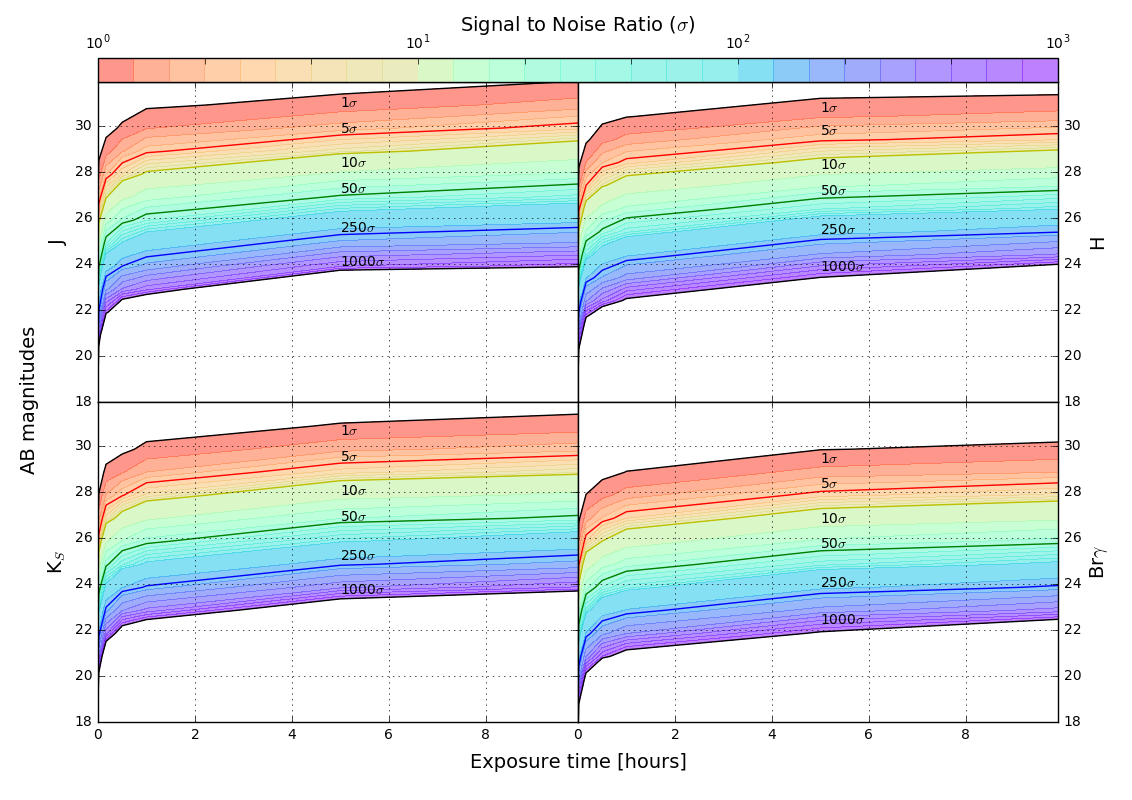
\includegraphics[width=\textwidth]{images/MICADO_SNR_Rainbow_JHKBrG_ab}
    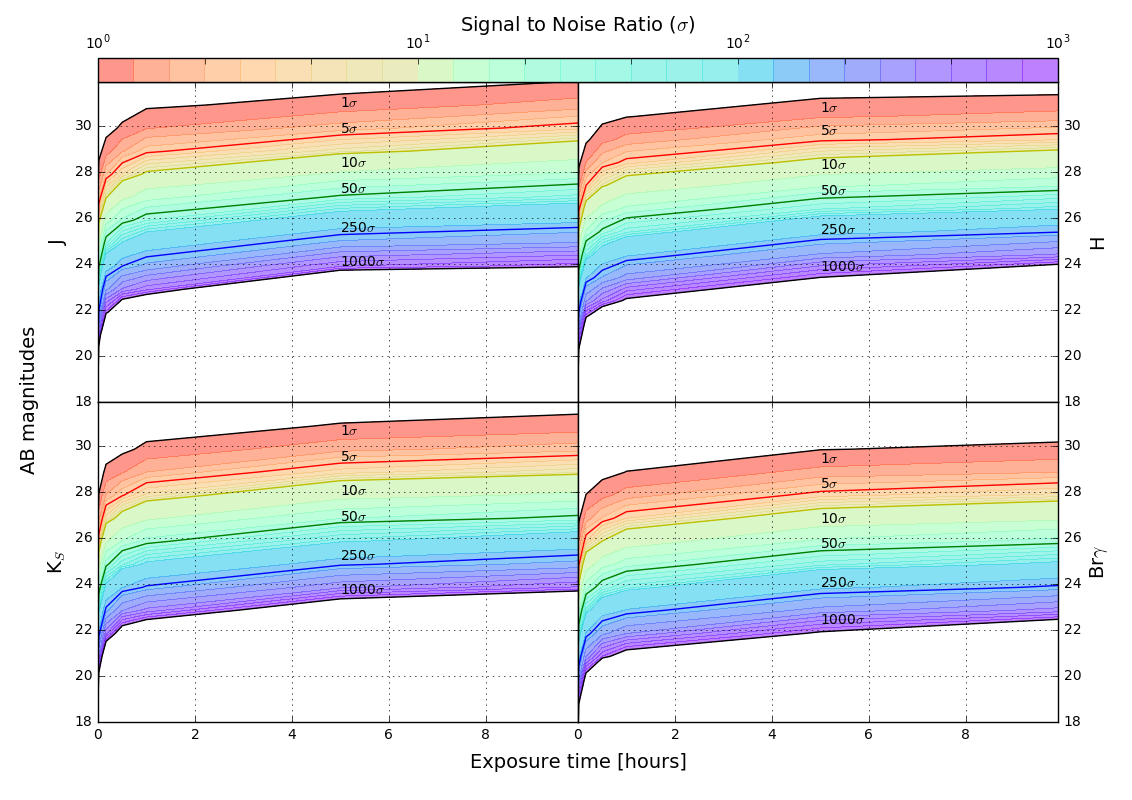
\includegraphics[width=\textwidth]{images/MICADO_SNR_Rainbow_JHKBrG_ab}

    \caption{Limiting magnitude plots for the wide field (4\,mas/pixel) imaging mode of MICADO at the ELT in Vega magnitudes.
    Signal-to-noise ratios above $5\sigma$ are sufficient for photometry.
    High precision astrometry requires stronger detections $\sim 250\sigma$.
    It should be noted that these magnitudes apply to the current design of MICADO and the ELT.
    At the time of publication MICADO is still in its design phase.
    As such we expect small changes in these values as the MICADO design matures.}
    
    \label{fig:point_source_sensitivities}
    
\end{figure*}


% 5hr  ETC JHK 28.7  27.9  27.5   M1 Area is 10% larger, but we used SCAO with 50% SR. They used wider filters, but higher BG
% 2.6s ETC JHK 23.6  23.1  22.5
% Sat  ETC JHK 15.8  15.6  14.9   M1 Area is 10% larger, pixels 5mas, SNR~750 After normalising they fit


% \begin{table*}

%     \centering
%     \caption{Specific point-source sensitivities for the NIR broadband filters J, H and Ks and the narrow band filter \brgamma. $5\sigma$ and $10\sigma$ are generally accepted detection limits for photometric measurements, while for accurate astrometry signal-to-noise ratios above $250\sigma$ are required. The errors on these magnitudes are $\pm 0.1$\m. It should be noted that these magnitudes apply to the current design of MICADO and the ELT. At the time of publication MICADO is still in its design phase. As such we expect small changes in these values as the MICADO design matures.}
%     \label{tbl:micado_point_source_sensitivities}

%     \begin{tabular}{ l r | r r r r r r r }
%         \hline\hline
% Filter          & SNR       & 2.6 sec & 10 sec    & 1 min     & 10 min    & 1 hr      &  5 hrs    & 10 hrs   \\
%         \hline
%                 & 5\sig     & 23.4\m  &   24.4\m  &   25.6\m  &   26.7\m  &   27.8\m  &   28.7\m  &   29.0\m   \\
%     J           & 10\sig    & 22.6\m  &   23.6\m  &   24.8\m  &   26.0\m  &   27.0\m  &   27.9\m  &   28.2\m   \\
%                 & 250\sig   & 18.7\m  &   19.9\m  &   21.1\m  &   22.4\m  &   23.4\m  &   24.2\m  &   24.6\m   \\
%         \hline
%                 & 5\sig     & 23.0\m  &   23.8\m  &   24.8\m  &   26.0\m  &   27.0\m  &   27.9\m  &   28.3\m   \\
%     H           & 10\sig    & 22.2\m  &   23.0\m  &   24.0\m  &   25.3\m  &   26.2\m  &   27.1\m  &   27.5\m   \\
%                 & 250\sig   & 18.6\m  &   19.4\m  &   20.4\m  &   21.7\m  &   22.7\m  &   23.5\m  &   23.9\m   \\ 
%         \hline
%                 & 5\sig     & 22.4\m  &   23.1\m  &   24.1\m  &   25.6\m  &   26.4\m  &   27.3\m  &   27.7\m   \\
%     Ks          &  10\sig   & 21.6\m  &   22.4\m  &   23.4\m  &   24.8\m  &   25.6\m  &   26.5\m  &   26.9\m   \\
%                 &  250\sig  & 18.0\m  &   18.9\m  &   19.8\m  &   21.0\m  &   22.1\m  &   22.9\m  &   23.3\m   \\
%         \hline
%                 & 5\sig     & 20.6\m  &   21.8\m  &   22.9\m  &   24.1\m  &   25.2\m  &   26.0\m  &   26.3\m   \\
%     \brgamma    & 10\sig    & 19.8\m  &   21.0\m  &   22.1\m  &   23.4\m  &   24.4\m  &   25.2\m  &   25.6\m   \\
%                 & 250\sig   & 16.0\m  &   17.1\m  &   18.4\m  &   19.8\m  &   20.8\m  &   21.7\m  &   22.1\m   \\
%         \hline
        

%     \end{tabular}
     
        
% \end{table*}

\begin{table}

    \centering
    \caption{Specific point-source sensitivities for the NIR broadband filters J, H and Ks and the narrow band filter \brgamma.
    The $5\sigma$ detection limits of a 5 hour exposure are given below in AB and Vega magnitudes and are valid for strehl ratios of 29\%, 51\%, and 68\% in the J, H and Ks filters.
    The errors on these magnitudes are $\pm 0.1$\m.}
    \label{tbl:micado_point_source_sensitivities}

    \begin{tabular}{ l | c c c c }
        \hline\hline
Filter          & J         & H        & Ks         & Br $\gamma$   \\
        \hline                
    AB          & 29.6\m    & 29.3\m   & 29.1\m     & 27.0\m        \\
        \hline                
    Vega        & 28.7\m    & 27.9\m   & 27.3\m     & 26.0\m        \\
        \hline                
    \end{tabular}

\end{table}


For studies of stellar populations, the detection limit is often set to $5\sigma$.
% , where $\sigma$ is the level of total background noise inside an aperture set around a star. 
Table~\ref{tbl:micado_point_source_sensitivities} lists MICADO's limiting magnitudes for the photometric case in the AB and Vega magnitude systems.
Fig. \ref{fig:point_source_sensitivities} shows a range of signal to noise ratios for various exposure times in the Vega system.
For an exposure time of 5\,hours, we find the limiting AB magnitudes in the main NIR broadband filters for a $5\sigma$ detection to be $J_{AB}=29.6$\m, $H_{AB}=29.3$\m and $K_{s  AB}=29.1$\m
. For the narrow-band filter \brgamma we find a limiting magnitude of $Br\gamma_{AB}=27.0$\m.
The J and H limiting magnitudes match those from the ELT exposure time calculator\footnote{\url{https://www.eso.org/observing/etc/bin/simu/elt_ima}} to within 0.1\m.
The Ks estimate is 0.2\m weaker than that from the ETC.

However, in order to achieve a high level of astrometric precision (e.g.\ down to levels of $\sim 1/30$th of a pixel, or $\sim 50\,\upmu\mathrm{as}$), a much higher signal-to-noise ratio is required, e.g.\ $\sim 250\sigma$ (D. Massari, private communication).
For astrometric purposes, we find a crude estimate of the limiting (Vega) magnitudes to be 24.2\m, 23.5\m, 22.9\m in J, H and Ks filters and 21.7\m in the \brgamma filter.
Here we have used the Vega system as it is more common within the astrometric community.
It should be strongly emphasised that there are a variety of external factors which heavily influence the accuracy of astrometric measurements, especially when using AO wavefront corrections, and therefore these estimates should be understood as rough limits for a best case scenario.
They are simply meant to inform the reader about the approximate brightness limits for astrometric observations, and should be treated appropriately.

Fig.~\ref{fig:point_source_sensitivities} shows SimCADOs estimate of the full range of limiting magnitudes for observations from the shortest integration time to a full 10\,hour observing program and for signal-to-noise ratios of $1\sigma$ to $1000\sigma$.
It is prudent to mention again that these estimates are applicable for an on-axis SCAO observation near the Zenith where the targets of interests are closer than $\sim5\arcsec$ from the SCAO reference star.

% \footnote{To convert to the AB system $\sim 0.9$, $\sim 1.4$ and $\sim 1.85$ should be added to the J, H and Ks magnitudes respectively.}

\subsection{Point source saturation limits}
\label{subsec:MICADO_saturation_limits}

\begin{table}

    \centering
    \caption{Saturation limits for MICADO assuming an effective detector well depth of $10^5\,\mathrm{e}^{-}/\mathrm{pixel}$.
    The shortest integration time for a full H4RG detector will be $\sim 2.6\,\mathrm{s}$ \citep{micado}.
    The limits are split between the two default imaging modes of MICADO: Wide-field mode (4\,mas/pixel, $\sim 50\arcsec$ FoV), and the zoom mode (1.5\,mas/pixel, $\sim 20\arcsec$ FoV).
    The brighter zoom mode saturation limit is due to the PSF distributing the point source flux over a larger amount of pixels.}
    %While the ESO exposure time calculator for the ELT has a slightly different configuration for the imaging mode, when the results are normalised we find that the SimCADO saturation limits are within 0.1\m of the ETC's limits.
    
    \label{tbl:micado_saturation}
    % \begin{tabular}{ l c | c c }
    %     \hline\hline
    % Filter      & DIT         & Wide field    & Zoom        \\
    %     \hline                              
    % J           & 2.6\,s      & 15.9\m        & 13.6\m      \\
                
    %     \hline                              
    % H           & 2.6\,s      & 15.6\m        & 13.4\m      \\
                
    %     \hline                              
    % K$_{s}$     & 2.6\,s      & 14.8\m        & 12.5\m      \\
                
    %     \hline                              
    % \brgamma    & 2.6\,s      & 12.0\m        & 9.9\m       \\
                
    %     \hline
    % \end{tabular}

    \begin{tabular}{ l l | c c c c}
        \hline\hline
    Pixel scale & Phot. Sys.    & J         & H         & K$_s$     & \brgamma  \\
        \hline                
    4 mas       & AB            & 16.8\m    & 17.0\m    & 16.6\m    & 13.0\m    \\
                & Vega          & 15.9\m    & 15.6\m    & 14.8\m    & 12.0\m    \\
        \hline
    1.5 mas     & AB            & 14.5\m    & 14.8\m    & 14.3\m    & 10.9\m    \\
                & Vega          & 13.6\m    & 13.4\m    & 12.5\m    & 9.9\m     \\
        \hline
    \end{tabular}

\end{table}

Given the ELT's collecting area of 978\,m$^2$, it is also important to know the saturation limits of the detectors when considering possible observational strategies.
Basic aperture photometry is only reliable when the maximum pixel values inside the aperture are within the linear regime of the detectors.
Advanced techniques such as PSF fitting will naturally allow this threshold to be extended.
However, given the unorthodox shape, the many sharp artefacts, and the dynamic nature of an AO corrected PSF for the ELT, the use of advanced photometric methods will prove challenging.
Therefore in order to set conservative limits on the accuracy of photometry for bright sources with MICADO we decided to define photometric reliability as stars with only unsaturated pixels.

The minimum read-out time for a full H4RG detector will be $\sim 2.6$\,seconds.
% MICADO will also offer a fast readout mode for windowed regions of the detector capable of reading out e.g. a $100\times 100$ pixel area at a rate of $200\,\mathrm{Hz}$ ($\mathrm{DIT} \sim 5\,\mathrm{ms}$). 
To calculate the bright star limits we took the brightest star from the simulated images that had no values over the correctable non-linear regime.
As there is little data publicly available for the performance of HAWAII-4RG detectors, we assumed their characteristics will be similar to the HAWAII-2RG chips.
According to \citet{hawaii2rg}, all detectors in the HAWAII-RG family have a correctable linearity regime (within 5\,\%) of $\sim 10^{5}\,\mathrm{e}^{-}/\mathrm{pixel}$ with a full well depth of $<1.5 \cdot 10^{5}\,\mathrm{e}^{-}\mathrm{pixel}^{-1}$.
Table~\ref{tbl:micado_saturation} shows the brightest magnitudes that can be observed in the J, H, Ks and \brgamma filters without any pixels saturating. 

As a sanity check, we compared the limits in Table~\ref{tbl:micado_saturation} to the saturation limits given by the ELT exposure time calculator provided by ESO.
The ETC uses a slightly different configuration for the imaging mode, the most notable differences being a collecting area of $1100\,\mathrm{m^2}$ and a plate scale of 5\,mas.
After rescaling the results from the ETC to match the values used in SimCADO (978\,m$^2$, 4\,mas/pixel), we find that SimCADO matches the ETC's calculations to within 0.1\m.
This is pleasantly surprising given the large number of assumptions built into the ETC.

It is worth noting that in the standard wide-field imaging mode with an integration time of 2.6\,s, MICADO will saturate around the detection limit of the 2MASS survey, i.e. (Vega) $J=15.8$\m, $H=15.1$\m and $K_{s}=14.3$\m \citep{2mass}.
On the one hand, this is a testament to the extreme increase in observing capabilities that the ELT and MICADO will provide.
On the other hand, this will prove problematic for observers as all telescope pointings within $\sim 25\arcsec$ of a 2MASS source will need to account for the effects of overly bright sources in the field of view.
Given that the diffraction spikes of the ELT's PSF are long and prominent, there is a good chance that they will cause issues with the reduction and analysis of fainter, more interesting regions. 


\subsection{Spectral type with distance}
\label{subsec:spec_type_vs_dist}

Four of the major science drivers for MICADO rely on determining the properties of stellar populations.
Hence we found it prudent to use the sensitivity estimates from SimCADO to calculate limiting distances for a $5\sigma$ detection for different spectral types.
Fig.~\ref{fig:MS_distances} shows the apparent magnitude of a selection of main-sequence stars with increasing distance as well as the sensitivity limits for MICADO for a range of exposure times.
We used the main sequence absolute magnitudes given in Table~5 of \citet{pecaut2013}\footnote{Additional information for the L and T dwarves not reported by Pecaut and Mamajek (2013) were taken from the associated website \url{http://www.pas.rochester.edu/~emamajek/EEM_dwarf_UBVIJHK_colors_Teff.txt}}.
As the brightest stars in the main sequence cover almost the same magnitude range as all giant and most supergiant stars, those readers interested in the limiting distances for stars that have left the main sequence are requested to use the distances for a main sequence star with an equivalent absolute magnitude. 

Using SimCADO we determined that MICADO should be able to detect all A-type stars in Centaurus~A at a distance of 4\,Mpc with a 5\,hour observation.
A 1\,hour observation should be sufficient to detect all stars down to the Hydrogen burning limit ($M < 0.08 M_{\odot}$) in the Magellanic Clouds ($\sim 50\,\mathrm{kpc}$).
However at this distance all stars brighter than B1V will saturate within the shortest exposure time ($\mathrm{DIT} =2.6\,\mathrm{s}$).
For more case specific distance limits based on the SimCADO limiting magnitudes, we direct the reader to Fig.~\ref{fig:MS_distances}.
The equivalent plot for the Ks filter is included in the Appendix.
These distance estimates are based on an ideal case scenario of an isolated star and the current design of the MICADO optical train.
Therefore Fig.~\ref{fig:MS_distances} should be understood as illustrating upper limits for the distance estimates.
For example, we have also assumed no extinction along the line of sight.
Nor have we taken into account the increased background levels in crowded field.
Both effects will undoubtedly reduce the distance estimated by varying amounts.
\cite{leschinski2020} discusses in greater detail the degree to which the level of crowding affects these distance estimates.


\begin{figure*}

    \centering
    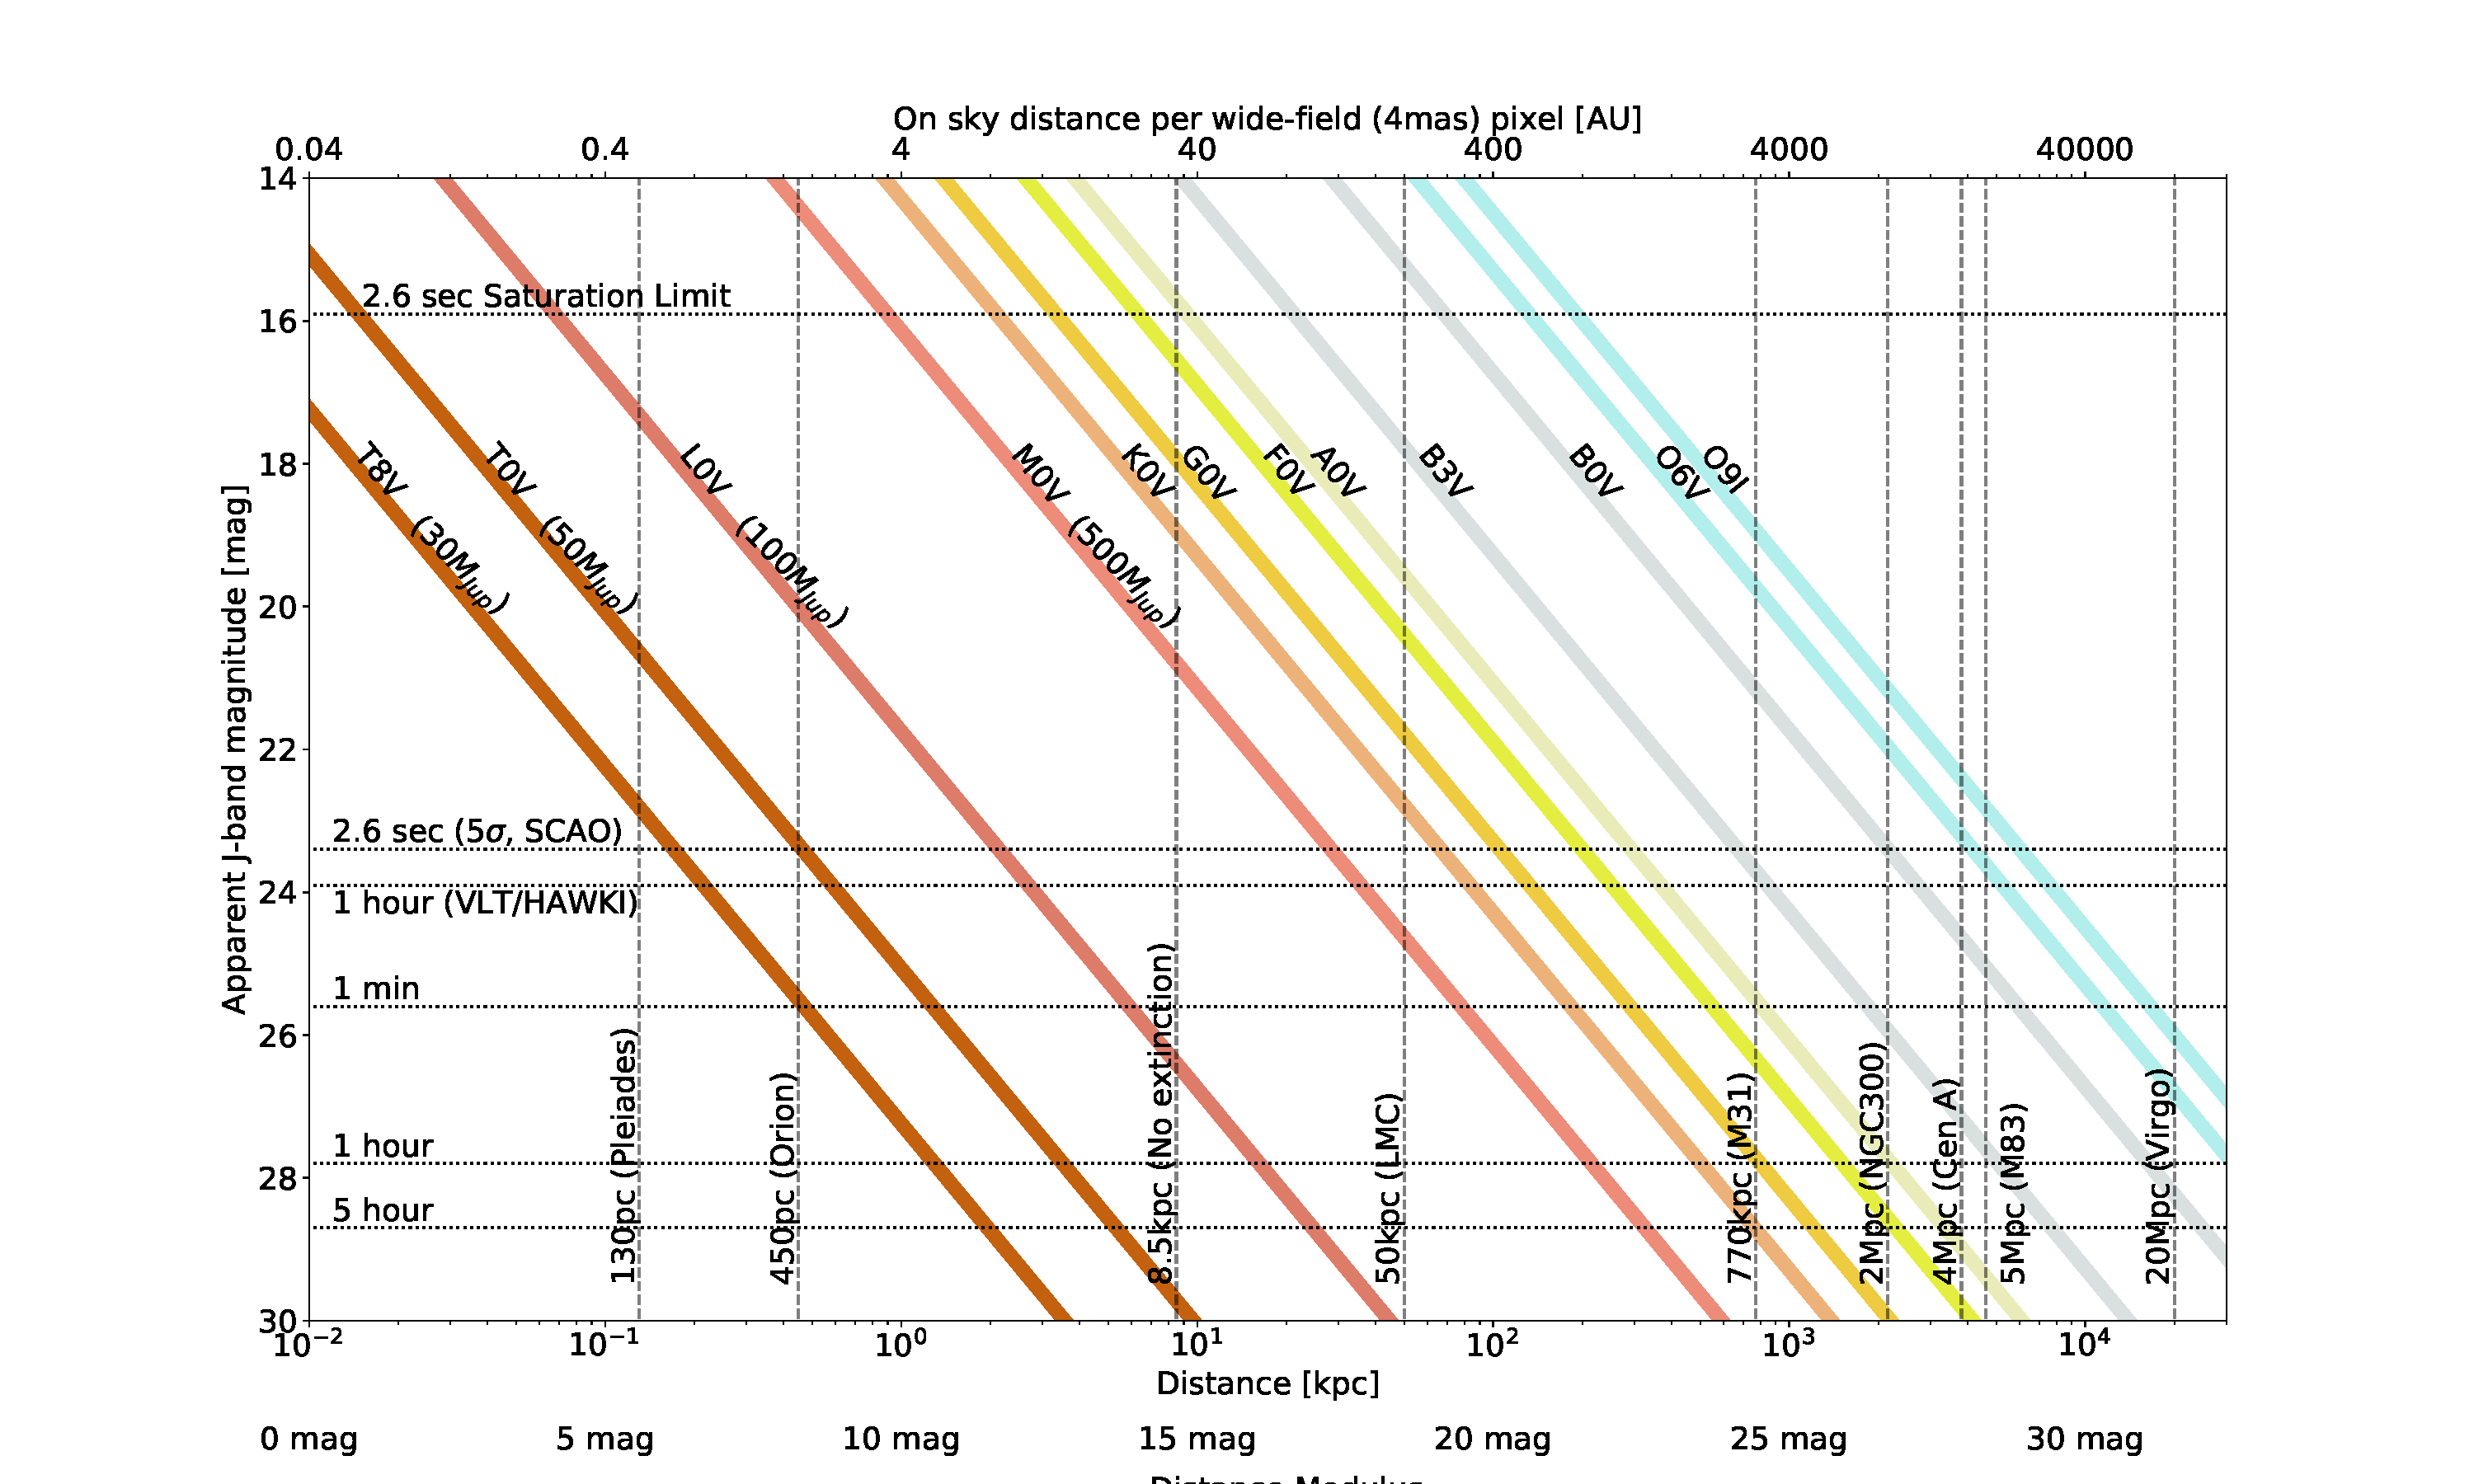
\includegraphics[width=\textwidth]{images/spec_type_vs_dist_J}

    \caption{The coloured lines represent the apparent magnitude of the major spectral types with increasing distance.
    The dashed horizontal lines, unless otherwise stated, represent the $5\sigma$ detection limits for various exposure times with MICADO.
    The intersection of a coloured line with a horizontal dotted line indicates that this type of main-sequence star will no longer be detectable by MICADO at the distance of the position of the intersection on the horizontal axis.
    As a reference, the dashed vertical lines show distances to well known astronomical objects. 
    % It is worth noting that what HAWK-I require 1\,hour to detect, will be detectable by MICADO in a minimum DIT (2.6\,seconds). While this comparison may seem ludicrous, the ELT has a primary mirror $\sim 20\times$ larger that of UT4 at the VLT and the smaller plate scale of MICADO means a factor of $\sim 35\times$ less background flux per pixel.
    }
    
    \label{fig:MS_distances}
    
\end{figure*}


\subsection{Accuracy of the SimCADO sensitivity predictions}
\label{subsec:MICADO_accuracy}

\begin{figure*}
    \centering
    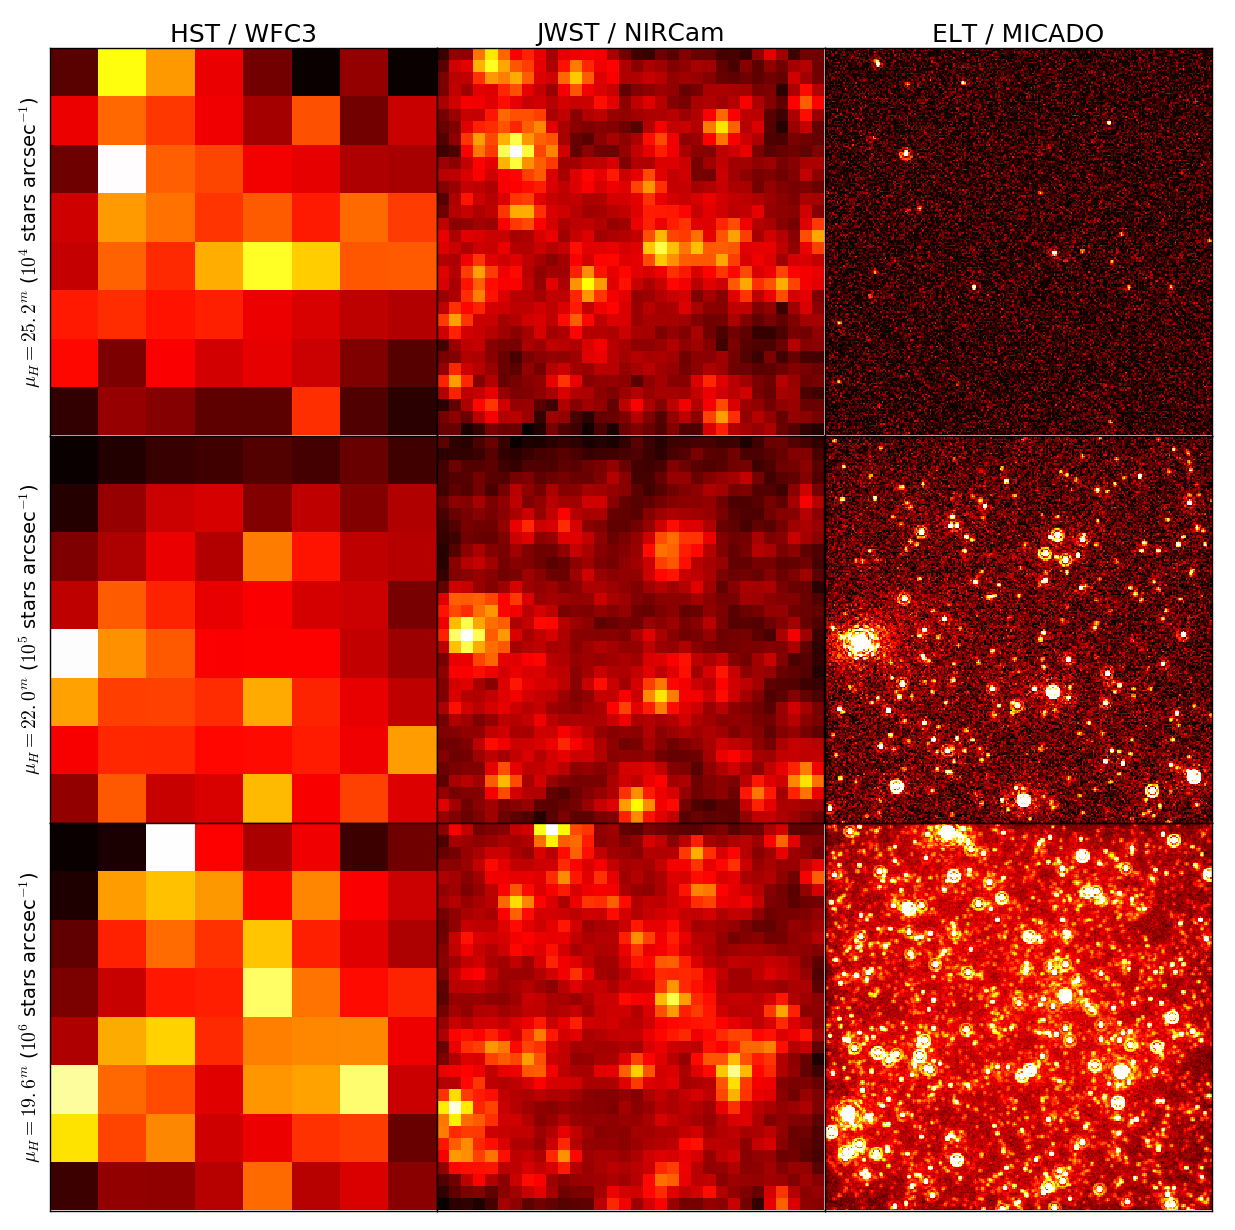
\includegraphics[width=\textwidth]{images/Virgo_old_stellar_pop_HST_JWST_ELT_H_band}
    
    \caption{An illustration of the improvement in resolution that MICADO will provide for observations of densely populated regions compared to HST and JWST.
    The three rows of 1"x1" images show the low (top, $\mu_H=25.2^m$), medium (centre, $\mu_H=22.0^m$) and high (bottom, $\mu_H=19.6^m$) surface brightness regions of an elliptical galaxy at a distance of 18 Mpc - approximately the distance of the Virgo cluster.
    These simulated images were created using configuration files for SimCADO which mimic the optical systems of HST/WFC3, JWST/NIRCam and ELT/MICADO.  
    }
    \label{fig:stellar_field_comp}

\end{figure*}

The accuracy of SimCADO simulations was verified by comparing simulated images with real HAWK-I observations.
Furthermore, estimates from SimCADO images of the detection and saturation limits for observations with MICADO fall within 0.1\m of the values given by the ELT exposure time calculator (after normalising the two optical train configurations).
These two results give us confidence that MICADO's sensitivity can be accurately predicted from simulations with SimCADO.
These simulations have however been conducted using several simplifications.
For example, the atmospheric conditions were assumed to mirror those of the average night at Paranal.
Given that the NIR sky background can vary up to $\sim 0.2$\m within 15\,minutes \citep{moreels08} and that it is also dependent on the level of water in the air as well as the airmass of the pointing, it is clear that the true detection limits of MICADO will vary from this first round of predictions with SimCADO.
Furthermore, the PSF used for the current round of SimCADO predictions was uniform across the field of view.
This will definitely not be the case.
Reductions in the Strehl ratio of $>50\,\%$ over the MICADO field of view are expected for SCAO observations \citep{clenet2015}.
Such variations will have a marked impact on sensitivity in the outer regions of the MICADO focal plane.
Readers interested in simulating observations at large distances (>10 arcsec) from a SCAO NGS are directed to look into the python package AnisoCADO (\url{https://anisocado.readthedocs.io/}) in conjunction with SimCADO.

Another challenge for estimating the performance of the telescope and instrument will be the ELT's PSF.
Accurate photometry of bright sources, extracting faint sources that are covered by the wings of the brighter sources, and accurate astrometry all rely on accurate knowledge of the shape of the PSF.
As can be seen in Fig.~\ref{fig:stellar_field_comp}, the segmented nature of the diffraction spikes of the SCAO PSF could easily confuse a star finding algorithm.
Additionally, the PSF will rotate with respect to the field over the course of an observing run due to the ELT's alt-azimuth mount.
Arguably though, this may prove advantageous as it will provide a natural rotational dithering, which may smooth out the sharp features of the PSF.
An alternative approach would be to deconvolve the images with a spatially varying model of the PSF.
This would however require multiple descriptions of the PSF for each detector frame, which could slowly become a challenging data management task.
Whether this task belongs in the automated data pipeline or is left to the user is still undecided.
A different approach would be to use a blind deconvolution algorithm \citep{vorontsov2017}.
Recent results are encouraging, although it remains to be seen how well this approach works for strong spatial variations in the PSFs.
In any case, the complex PSF of the ELT will present a challenge to standard data analysis techniques.
How the PSF artefacts of bright stars affect the surrounding environment is a question that should be considered in the earliest stages when planning observations with the ELT and MICADO.

\section{Future functionality for SimCADO}
\label{sec:future}

The results of the first verification run show that SimCADO is capable of recreating observations with only descriptions of the optical elements as input.
There are, however, still several aspects that require attention by the development team.
In short they are:

\paragraph{Atmospheric variations:}
SimCADO uses a set of standardised spectra from SkyCalc, scaled to the required background level, to provide the sky background flux for any chosen filter.
Currently this atmospheric spectrum is independent of the atmospheric water content (PWV\,=\,2.5\,mm), however it does reflect the airmass.
For the verification run described here, these points were not relevant: the archival data for M\,4 were taken close to zenith and the image of NGC\,4147 (airmass $\sim 1.44$) was primarily used as a control for its different exposure length.
Functionality to directly connect SimCADO to the ESO SkyCalc service using the SkyCalc-iPy python package (\url{https://skycalc-ipy.readthedocs.io}) will be included in the next release.
This will enable the effects of different atmospheric conditions to be include on-the-fly in simulations.

\paragraph{PSF variability:}
While not as important for a seeing-limited instrument, the variations in the shape of the PSF over the field of view for observations conducted with adaptive optics is not a trivial effect.
We recently added the functionality to include the effects of a field-varying PSFs for the SCAO observation mode over the full field of view in simulations.
The currently available set of SCAO PSFs was generated by the AnisoCADO tool.
Field-varying MCAO PSFs are not yet available to the public.
It should be noted that the exposure times are assumed to be long enough that the PSF should not vary significantly between exposures (EXPTIME \textgreater 5\,s).
Whether or not this assumption holds for all time scales remains to be investigated.

\paragraph{Distortion effects:}
For photometric studies optical distortions are a nuisance.
For astrometric studies they are critical.
SimCADO includes the functionality to shift point sources on the sub-pixel level.
As such we are currently investigating the best way to implement the use of distortion maps in the model of the optical train.

\paragraph{Non-common path aberrations:} Only the effective loss in flux due to PSF broadening from the combined set of NCPAs is currently included in SimCADO.
This is a function of wavelength and as such can be modelled effectively as an additional transmission curve.
The spatial aspects of the NCPAs in the context of the MICADO optical train are currently being investigated, however a first order approximation of the spatial effects is already included in the current development version of the code.

\paragraph{Spectroscopy:} MICADO has been designed to also include optics for a long slit spectrograph.
A separate python package, SpecCADO, using the core functionality of SimCADO was created to model the more complex spectroscopy mode\footnote{\url{https://homepage.univie.ac.at/oliver.czoske/}}.
The extended functionality of SpecCADO will be merged into a future release version of SimCADO.

Although there is still much work to do, SimCADO is already capable of simulating raw detector read-outs for each of the MICADO imaging modes, using both the SCAO and MCAO adaptive optics configurations.
This alone covers the majority of the primary science drivers for MICADO.
It should also be noted that MICADO is still in the design phase and so the composition of the optical train, and therefore the default data installed alongside SimCADO, are likely to change in the future.
However, given the maturity of the design we foresee no radical changes to the optical system, and thus no radical changes to the sensitivity estimates presented in this paper.


\section{Summary}
\label{sec:conclusions}

As part of the design activities for the MICADO instrument we have developed an instrument data simulator in Python: SimCADO.
The software is capable of generating detector frames for any given optical train configuration and source object description.
A brief summary of our activities and results are listed below:

\begin{itemize}

    \item In conjunction with the MICADO instrument team we have developed a modular python package that allows us to model each element in the optical train separately.
    The software allows the user to fully control the configuration of the optical train as well as the description of the astronomical object to be observed.
    Images produced by the package are in the standard FITS format and can be treated as coming directly from a telescope.
    
    \item We configured SimCADO to mimic the UT4/HAWK-I optical train and ``observed'' two globular clusters with this setup.
    A comparison to archive data for the same globular clusters showed that SimCADO is capable of reproducing all the major and most of the minor effects that are seen in raw detector frames from HAWK-I.
    A photometric comparison shows a one-to-one correlation between the flux observed in the archive and simulated images.
    Although there is scatter around this line, the primary source of uncertainty lies with the photometric analysis of the archive data and not with the simulated images.
    Additionally SimCADO is able to reproduce the detection limits given by the ESO exposure time calculator for a 1-hour observation with HAWK-I.
    
    \item Using the configuration for the ELT/MICADO optical train we simulated a grid of stars to find the detection limits for different exposure times.
    We have shown that the 5\,hour 5$\sigma$ detection limits in AB (Vega) magnitudes are: $J=29.6$\m ($28.7$\m), $H=29.3$\m ($27.9$\m) and $K_{s}=29.1$\m ($27.3$\m), while the saturation limit for the shortest exposure time ($\mathrm{MINDIT}=2.6\,\mathrm{s}$) in the wide-field (4\,mas/pixel) mode are similar to the 2MASS detection limits (Vega): $J=15.9$\m, $H=15.6$\m and $K_{s}=14.8$\m.
    The use of the zoom mode (1.5\,mas/pixel) in conjunction with a narrow band filter, such as the \brgamma filter, would increase this limit to $\sim 9.9$\m (Vega).

    \item With these detection limits we have shown that MICADO will be capable of detecting individual A0\,V stars at a distance of 4\,Mpc (Centaurus~A), while any star brighter than B1\,V at a distance of 50\,kpc (LMC) will saturate during the a single minimum length exposure.
    
    \item We will be adding the following functionality to SimCADO in the near future: a long slit spectrographic mode, MCAO field variable PSFs, variations in atmospheric conditions.

\end{itemize}

We encourage anyone who may want to use the ELT and MICADO for future observations to use SimCADO to simulate their science case in advance.
Not only will this help the community to get a feel for what MICADO will be capable of and where possible problems with an observing strategy will be, feedback from users will help us to develop the software in such a way as to meet the needs of the astronomical community.

\begin{acknowledgements}

SimCADO incorporates Bernhard Rauscher's HxRG Noise Generator package for python \citep{nghxrg}. 
This research made use of POPPY, an open-source optical propagation Python package originally developed for the James Webb Space Telescope project \citep{poppy}. 
This research made use of Astropy, a community-developed core Python package for astronomy \citep{astropy, astropy2}. 
This research made use of Photutils \citep{photutils}. 
This research has made use of ``Aladin sky atlas'' developed at CDS, Strasbourg Observatory, France \citep{aladin, aladinlite}.
SimCADO makes use of atmospheric transmission and emission curves generated by ESO's SkyCalc service, which was developed at the University of Innsbruck as part of an Austrian in-kind contribution to ESO. 
Based on data obtained from the ESO Science Archive Facility under request number Leschinski, \#331857.
This publication makes use of data products from the Two Micron All Sky Survey, which is a joint project of the University of Massachusetts and the Infrared Processing and Analysis Center/California Institute of Technology, funded by the National Aeronautics and Space Administration and the National Science Foundation \citep{2mass}.

This research is partially funded by the project IS538003 of the Hochschulraumstrukturmittel (HRSM) provided by the Austrian Government and administered by the University of Vienna. 
The authors would also like to thank all the members of the consortium for their effort in the MICADO project, and their contributions to the development of this tool.

\end{acknowledgements}

\bibliographystyle{aa}
\bibliography{simcado_refs}

\appendix
\section{Distance estimates for main sequence stars in Ks filter}

\begin{figure*}

    \centering
    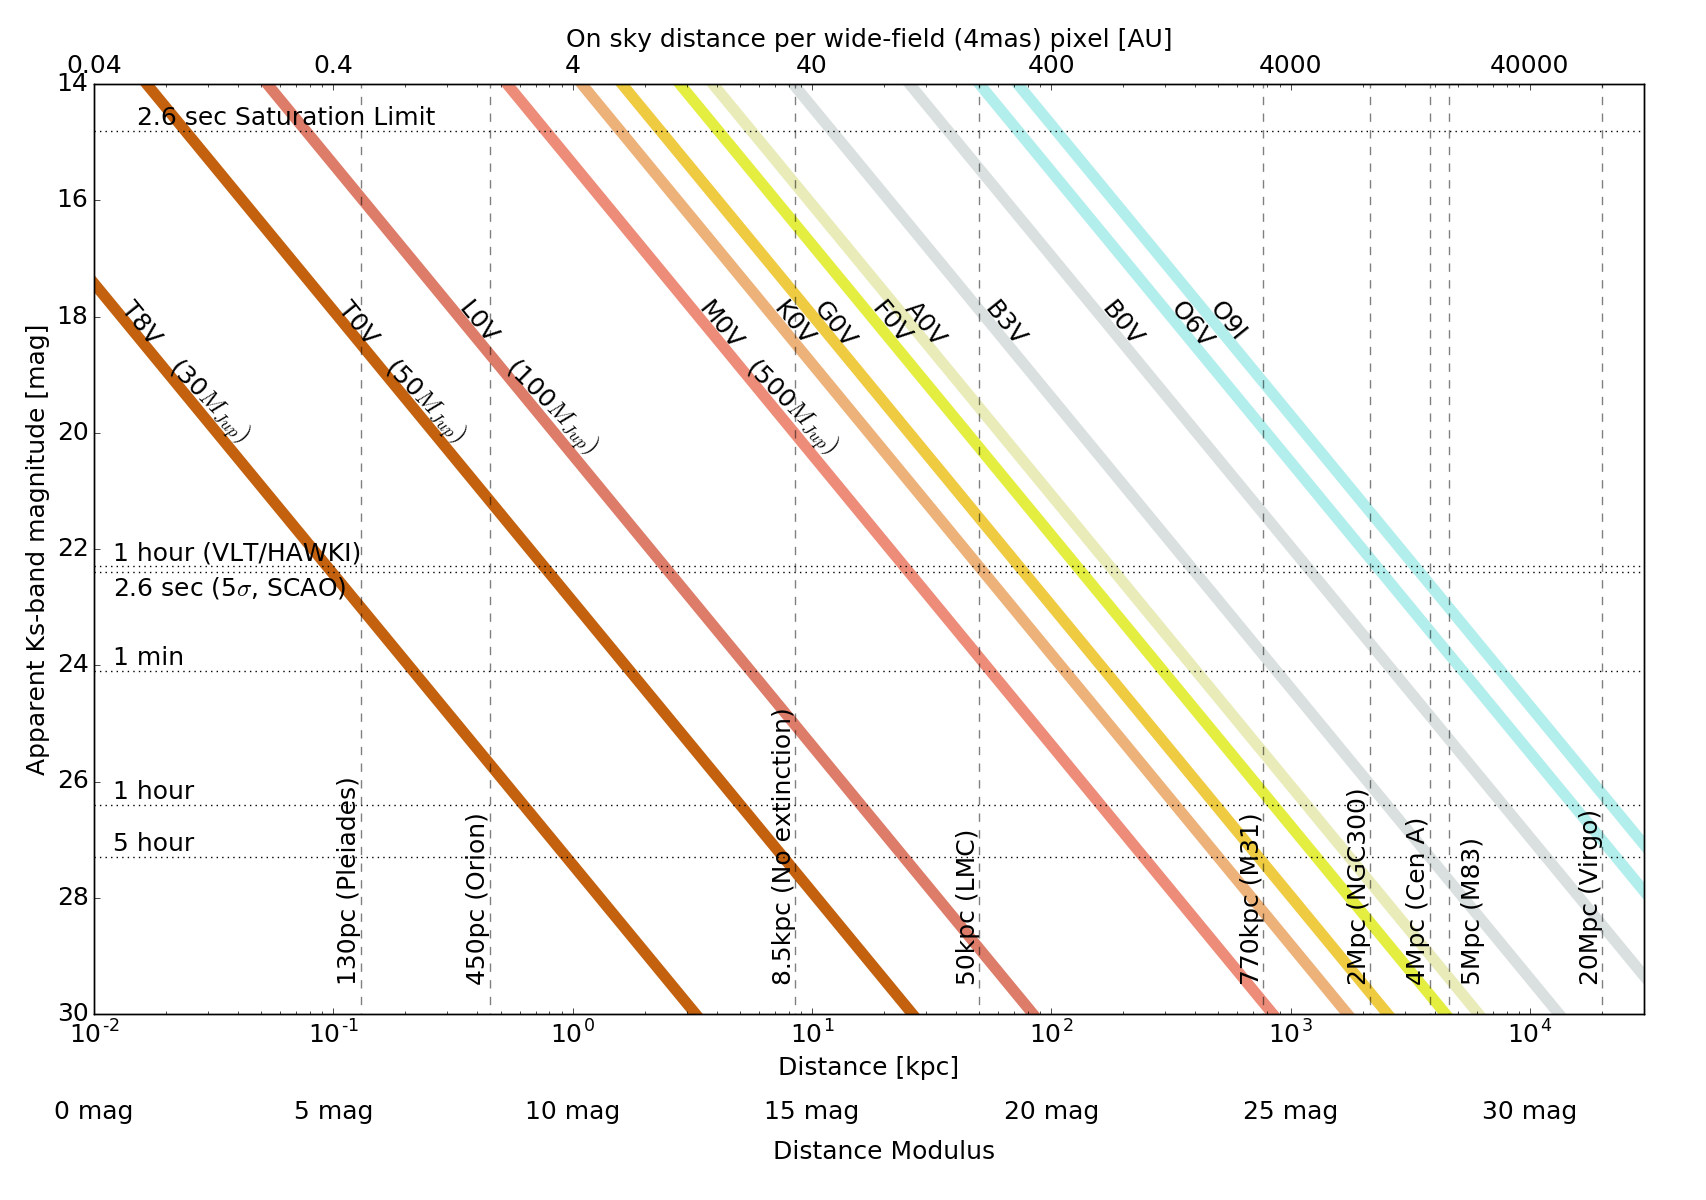
\includegraphics[width=\textwidth]{images/spec_type_vs_dist_paper2_Ks}
    
    \caption{The Ks-band equivalent of Fig.~\ref{fig:MS_distances}. As described in Fig.~\ref{fig:MS_distances} the coloured lines represent the apparent magnitude of the major spectral types with increasing distance. The dashed horizontal lines, unless otherwise stated, represent the $5\sigma$ detection limits for various exposure times with MICADO. When a coloured line crosses below a horizontal line, it means that this type of main sequence star will no longer be detectable by MICADO at the distance when the cross occurs. As a reference the dashed vertical lines show distances to well known astronomical objects.}
    
    \label{fig:MS_distances_Ks}
    
\end{figure*}


% \section{Comparison of the HAWK-I and MICADO configuration files}

% Although the SimCADO package is in the public domain, it currently does not have a software licence. Nevertheless we encourage anyone interested in simulating future ELT/MICADO observations to use SimCADO and to report any bugs to the authors. In the interests of transparency and reproducibility, we have included the configuration files that we used to generate SimCADO models of both the HAWK-I and MICADO optical trains. We are also willing to share any of the data files that subsequent users may need in order to reproduce our results. Please contact the authors directly. The software can be found at \url{www.univie.ac.at/simcado}


% \subsection{The MICADO configuration file}
% \label{appendix:micado_config}

% The standard configuration file used for the MICADO wide-field (4\,mas plate scale) imaging mode.

% \input{images/default.config}


% \subsection{The HAWKI configuration file}

% Rather than listing the full configuration for SimCADO as in Sect.~\ref{appendix:micado_config}, we simply list the parameters that were changed in order to create an optical train for UT4/HAWKI at the VLT.

% \input{images/hawki.config}


% \section{Settings for the HxRG Noise Generator script}

% In order to generate a stack of noise frames, SimCADO uses the python package NGHxRG. We have modified the values to reflect the characteristics of the new HAWAII-4RG chips that will be used in MICADO. The settings used by SimCADO are listed below:


% \begin{table*}
    % \centering
    % \begin{tabular}{|l|c|l|}
        % \hline
        % Noise Parameter             & Default Value & Description \\
        % \hline
        % White noise                 & 4 e-  & Standard deviation of read noise in electrons \\
        % Correlated pink noise       & 3 e-  & Standard deviation of correlated 1/f noise \\
        % Uncorrelated pink noise     & 1 e-  & Standard deviation of correlated 1/f noise \\
        % Alternating column noise    & 0.5 e$^-$ & Standard deviation of alternating column noise \\
        % Pedestal noise              & 4   e$^-$ & Level of pedestal drift in electrons \\
        % Number of read out channels & 64    &  \\
        % Number of row overheads     & 8     &  \\
        % Dead pixels                 & 1\%   & Percentage of pixels that are either ''hot'' or dead \\
        % Dead lines                  & 1\%   & Percentage of lines that are either ''hot'' or dead \\
        % \hline
    % \end{tabular}
    
    % \caption{Settings used by the HxRG noise generator code to model the read-out noise of the future MICADO detectors. See \citet{nghxrg} for more details.}
    % \label{tab:nghxrg}
    
% \end{table*}



%________________________________________________________________

\end{document}